\subsection{Syntactic Sugar}
\begin{frame}[fragile]{Parallel Operators}
\begin{lstlisting}[frame=htrbl]
(|***|) :: arr a b -> arr c d -> arr (a, c) (b, d)
(|***|) = parEval2 ()
\end{lstlisting}
\begin{center}
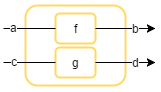
\includegraphics[scale=0.5]{images/starstarstar}
\hspace{2em}
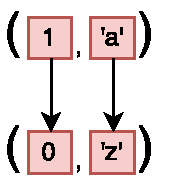
\includegraphics[scale=0.5]{images/parEval2}
\end{center}
\begin{lstlisting}[frame=htrbl]
(|&&&|) :: arr a b -> arr a c -> arr a (b, c)
(|&&&|) f g = (arr $ \a -> (a, a)) >>> f |***| g
\end{lstlisting}
\begin{center}
	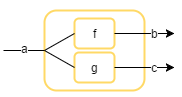
\includegraphics[scale=0.5]{images/dollardollardollar}
	\hspace{2em}
	\includegraphics[scale=0.5]{images/pardollardollardollar}
\end{center}
\end{frame}

\begin{frame}[fragile]{Parallelism made easy}
Parallel Evaluation made easy:
\begin{lstlisting}[frame=htrbl]
add :: Arrow arr => arr a Int -> arr a Int -> arr a Int
add f g = (f |&&&| g) >>> arr (\(u, v) -> u + v)
\end{lstlisting}
\begin{center}
	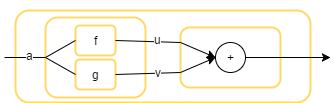
\includegraphics[scale=0.6]{images/addA-comb}
	\hspace{2em}
	\includegraphics[scale=0.5]{images/parAddA}
\end{center}
\end{frame}